\chapter{Biosignale}

Ein Signal ist nach DIN 44300 die Darstellung einer Nachricht/Information durch eine physikalische Grösse. Signale sind im allgemeinen Funktionen der Zeit, d.h. Signaländerungen treten im Laufe der Zeit auf. Sie können aber auch von anderen Parametern abhängen (z.B. dem Ort). Ein Signal kann also durch seine Amplitude (maximale Auslenkung) und seine Frequenz (Änderung pro Sekunde) beschrieben werden.
Ein lebender Organismus erzeugt autonom Biosignale. Biosignale sind energetisch-stofflich messbare physikalische Grössen. Weitere Biosignale können provoziert werden. Die Information wird über ein physikalisches/physiologisches Trägermedium übertragen. Abbildung \ref{fig:biosignale} zeigt eine Übersicht über die verschiedenen Biosignale.

\begin{figure}[h!]
\centering
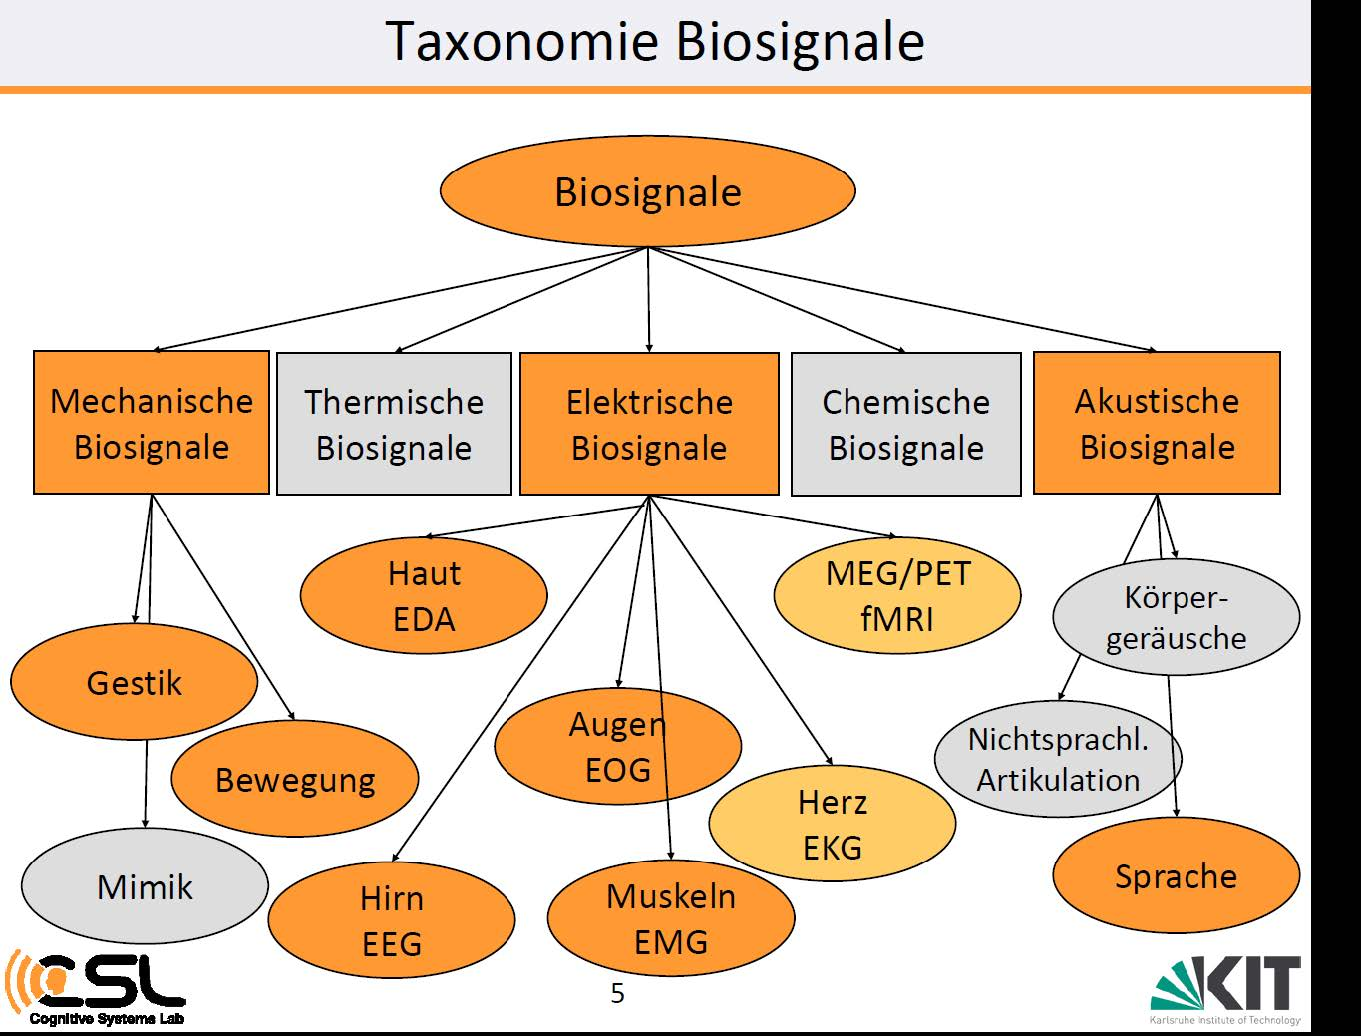
\includegraphics[width=0.6\linewidth]{fig/biosignale}
\caption{Taxonomie Biosignale}
\label{fig:biosignale}
\end{figure}

Nachfolgend einige Anforderungen die an einen Messaufnehmer gestellt werden:
\begin{itemize}
	\item Keine Beeinflussung derMessung/Rückwirkungsfreie Erfassung der Biosignale
	\item Elektrode sollte sehr klein sein (Mikroelektrode) , geringe Masse, geringes Volumen
	\item Hohe Stromdichte
	\item Kleiner Widerstand
	\item Geringes Rauschen
	\item hohe Toleranz bzgl. Artefakte
	\item Möglichst geringe Belastung des Patienten/Probanden
	\item Konstantes Übertragungsverhalten
	\item \dots
\end{itemize}
Auftretende Artefakte im Signal müssen durch Störungsunterdrückung herausgefiltert werden.